%% -*- coding:utf-8 -*-
\chapter{Yoneda's lemma}
\label{sec:yoneda}
Yoneda lemma is a fact about so called Hom functors. We will start
with the definition and examples for both
\mynameref{def:cov_hom_functor} and \mynameref{def:con_hom_functor}. The
definition and examples for Yoneda lemma will be provided after that. 
In the chapter we will assume that the category $\cat{C}$ to be a
\mynameref{def:localy_small_category}.

\section{Hom functors}

We are going to define the Hom functors. There are 2 hom functors:
\mynameref{def:covariant_functor} and
\mynameref{def:contravariant_functor}. For the
\mynameref{def:cov_hom_functor} we pick up an object $a$ from 
$\cat{C}$ and consider the collection of morphisms from $a$ to an
arbitrary object $x$ from the category. The collection is a
\mynameref{def:set} as soon as $\cat{C}$ is a
\mynameref{def:localy_small_category}. Therefore we can associate a
set (object from \mynameref{def:setcategory}) with the object $x$ from the
category $C$. 

The same approach is used for 
\mynameref{def:con_hom_functor}. But in the case we consider set of
morphisms from an arbitrary object $x$ to the picked object $a$ i.e.
we revert \mynameref{def:arrow}s in the case.

\subsection{Covariant Hom functor}
\begin{definition}[Covariant Hom functor]
\label{def:cov_hom_functor}
\index{Hom Functor!definition}
Let $\cat{C}$ is a \mynameref{def:localy_small_category} and $a \in
\catob{C}$. Consider \mynameref{def:functor} from $\cat{C}$ to the
\mynameref{def:setcategory} defined by the following rules
\begin{itemize}
\item $\forall x \in \catob{C}$ define an object in the set category:
  $\catmset[C]{a}{x} \in \catob{Set}$ 
\item $\forall f: x \to y \in \cathom{C}$ define a function in the set category
  $\catmset[C]{a}{f}: \catmset[C]{a}{x} \to \catmset[C]{a}{y}$ as follows
  $\catmset[C]{a}{f} = \{f \circ g | g \in \catmset[C]{a}{x}\}$.
\end{itemize}  
The \textit{covariant Hom functor} is denoted as $\catcovhom{C}{a}$.
\end{definition}

\begin{example}[Covariant Hom functor]
\label{ex:cov_hom_functor}
  \begin{figure}
    \centering
    \begin{tikzpicture}[ele/.style={fill=black,circle,minimum
          width=.8pt,inner sep=1pt},every fit/.style={ellipse,draw,inner
          sep=-2pt}]

      % the texts
      \node at (-2,4) {$\cat{C}$};        

      \node[ele,label=right:$a$] (a) at (0,1.5) {};    
      \node[ele,label=below:$b$] (b) at (0,3) {};    
      \node[ele,label=above:$c$] (c) at (0,0) {};
      \node[ele,label=left:$d$] (d) at (1.5,3) {};

      \draw[->,thick,shorten <=2pt,shorten >=2pt] (a) to
           [out=135,in=-135,looseness=20] node[left] {$\idm{a}$}
           (a); 

      \draw[->,thick,shorten <=2pt,shorten >=2pt] (b) to
           [out=135,in=45,looseness=20] node[above] {$\idm{b}$}
           (b); 

      \draw[->,thick,shorten <=2pt,shorten >=2pt] (c) to
           [out=-135,in=-45,looseness=20] node[below] {$\idm{c}$}
           (c); 

      \draw[->,thick,shorten <=2pt,shorten >=2pt] (d) to
           [out=45,in=-45,looseness=20] node[right] {$\idm{d}$}
           (d); 

      \draw[->,thick,shorten <=2pt,shorten >=2pt] (a) to
           [out=135,in=-135,looseness=0.5] node[left] {$f^{(b)}_1$}
           (b); 
      \draw[->,thick,shorten <=2pt,shorten >=2pt] (a) to
           [out=45,in=-45,looseness=0.5] node[right] {$f^{(b)}_2$} (b); 

      \draw[->,thick,shorten <=2pt,shorten >=2pt] (a) to
           [out=-135,in=135,looseness=0.5] node[left] {$f^{(c)}_1$}
           (c); 
      \draw[->,thick,shorten <=2pt,shorten >=2pt] (a) to
           [out=-45,in=45,looseness=0.5] node[right] {$f^{(c)}_2$}
           (c); 

      \draw[->,thick,shorten <=2pt,shorten >=2pt] (b) to
           [out=190,in=-190,looseness=2] node[left] {$f$} (c); 


      \draw[->,thick,shorten <=2pt,shorten >=2pt] (a) to
           [out=10,in=-10,looseness=3] node[right] {$g_1$}
           (c); 
      \draw[->,thick,shorten <=2pt,shorten >=2pt] (a) to
           [out=10,in=-10,looseness=5] node[right] {$g_2$}
           (c); 


      \node[draw,fit= (a) (b) (c) (d),minimum width=6cm, minimum
        height=5.5cm] {} ;

    \end{tikzpicture}
    \caption{Covariant Hom functor $\catcovhom{C}{a}$ example.
      Category $\cat{C}$} 
    \label{fig:cov_hom_functor}
  \end{figure}
Consider category $\cat{C}$ in the \cref{fig:cov_hom_functor}. It
consists of 4 objects: 
\[
\catob{C} = \{a,b,c,d\}.
\]
We are
going to construct $\catcovhom{C}{a}$ functor and therefore are
interested in the following sets of morphisms: 
\begin{eqnarray}
\catmset[C]{a}{a} = \{\idm{a}\},
\nonumber \\
\catmset[C]{a}{b} = \{f_1^{(b)}, f_2^{(b)}\}, 
\nonumber \\
\catmset[C]{a}{c} = \{f_1^{(c)}, f_2^{(c)}, g_1 = f \circ f_1^{(b)},
g_2 = f \circ f_2^{(b)}\}, 
\nonumber \\
\catmset[C]{a}{d} = \emptyset.
\nonumber
\end{eqnarray}
There is also a single \mynameref{def:morphism} $f$ between $b$ and $c$.

  \begin{figure}
    \centering
    \begin{tikzpicture}[ele/.style={fill=black,circle,minimum
          width=.8pt,inner sep=1pt},every fit/.style={ellipse,draw,inner
          sep=-2pt}]

      % the texts
      \node at (-2,4) {$\cat{Set}$};        

      \node[ele,label=right:$a'$] (a) at (0,1.5) {};    
      \node[ele,label=below:$b'$] (b) at (0,3) {};    
      \node[ele,label=above:$c'$] (c) at (0,0) {};
      \node[ele,label=right:$\emptyset$] (d) at (1.5,1.5) {};

      \draw[->,thick,shorten <=2pt,shorten >=2pt] (a) to
           [out=135,in=-135,looseness=20] node[left] {$\idm{a'}$}
           (a); 

      \draw[->,thick,shorten <=2pt,shorten >=2pt] (b) to
           [out=135,in=45,looseness=20] node[above] {$\idm{b'}$}
           (b); 

      \draw[->,thick,shorten <=2pt,shorten >=2pt] (c) to
           [out=-135,in=-45,looseness=20] node[below] {$\idm{c'}$}
           (c); 


      \draw[->,thick,shorten <=2pt,shorten >=2pt] (b) to
           [out=190,in=-190,looseness=2] node[left] {$f'$} (c); 


      \node[draw,fit= (a) (b) (c) (d),minimum width=6cm, minimum
        height=5.5cm] {} ;

    \end{tikzpicture}
    \caption{Covariant Hom functor $\catcovhom{C}{a}$ example. Category $\cat{Set}$}
    \label{fig:cov_hom_functor_set}
  \end{figure}

The corresponding
objects in the \mynameref{def:setcategory} is described in the
\cref{fig:cov_hom_functor_set}: 
\begin{eqnarray}
a' = \catmset[C]{a}{a} = \{\idm{a}\},
\nonumber \\
b' = \catmset[C]{a}{b} = \{f_1^{(b)}, f_2^{(b)}\}, 
\nonumber \\
c' = \catmset[C]{a}{c} = \{f_1^{(c)}, f_2^{(c)}, g_1, g_2\}, 
\nonumber \\
d' = \catmset[C]{a}{d} = \emptyset.
\nonumber
\end{eqnarray}

The $\catcovhom{C}{a}$ does the following mapping between objects:
\begin{eqnarray}
a \tof \catmset[C]{a}{a} = a',
\nonumber \\
b \tof \catmset[C]{a}{b} = b', 
\nonumber \\
c \tof \catmset[C]{a}{c} = c', 
\nonumber \\
d \tof \catmset[C]{a}{d} = \emptyset.
\nonumber
\end{eqnarray}
The functor maps morphisms in addition to objects. There are mapping
for trivial \mynameref{def:id}s: 
\begin{eqnarray}
\idm{a} \tof \idm{a'},
\nonumber \\
\idm{b} \tof \idm{b'},
\nonumber \\
\idm{c} \tof \idm{c'},
\nonumber \\
\idm{d} \tof \idm{\emptyset},
\nonumber
\end{eqnarray}
and for a single non trivial morphism $f \tof f'$ that is defined by
the following rules:
\begin{eqnarray}
f'(f_1^{(b)}) = g_1,
\nonumber \\
f'(f_2^{(b)}) = g_2,
\nonumber
\end{eqnarray}
i.e. the \mynameref{def:function_image} of $f'$ is a subset of
$\catmset[C]{a}{c}$:
\[
\Ima{f'} \subsetneq \catmset[C]{a}{c}.
\]
\end{example}

\subsection{Contravariant Hom functor}
If we revert \mynameref{def:arrow}s in the \cref{def:cov_hom_functor} then we can get
a definition for \mynameref{def:contravariant_functor} as follows.
\begin{definition}[Contravariant Hom functor]
\label{def:con_hom_functor}
Let $\cat{C}$ is a \mynameref{def:localy_small_category} and $a \in
\catob{C}$. Consider \mynameref{def:functor} from $\cat{C}$ to the
\mynameref{def:setcategory} defined by the following rules
\begin{itemize}
\item $\forall x \in \catob{C}$ define an object in the set category:
  $\catmset[C]{x}{a} \in \catob{Set}$ 
\item $\forall h: x \to y \in \cathom{C}$ define a function in the set category
  $\catmset[C]{h}{a}: \catmset[C]{y}{a} \to \catmset[C]{x}{a}$ as follows
  $\catmset[C]{h}{a} = \{g \circ h | g \in \catmset[C]{y}{a}\}$.
\end{itemize}  
The \textit{contravariant Hom functor} is denoted as $\catconhom{C}{a}$.
\end{definition}

From the definition of \mynameref{def:contravariant_functor} follows
that we can get it simply reverting \mynameref{def:arrow}s in the initial category. 
Lets do it for \cref{ex:cov_hom_functor} as follows
\begin{example}[Contravariant Hom functor]
\label{ex:con_hom_functor}
  \begin{figure}
    \centering
    \begin{tikzpicture}[ele/.style={fill=black,circle,minimum
          width=.8pt,inner sep=1pt},every fit/.style={ellipse,draw,inner
          sep=-2pt}]

      % the texts
      \node at (-2,4) {$\cat{D}$};        

      \node[ele,label=right:$a$] (a) at (0,1.5) {};    
      \node[ele,label=above:$b$] (b) at (0,0) {};    
      \node[ele,label=below:$c$] (c) at (0,3) {};
      \node[ele,label=left:$d$] (d) at (1.5,0) {};

      \draw[->,thick,shorten <=2pt,shorten >=2pt] (a) to
           [out=135,in=-135,looseness=20] node[left] {$\idm{a}$}
           (a); 

      \draw[->,thick,shorten <=2pt,shorten >=2pt] (b) to
           [out=-135,in=-45,looseness=20] node[below] {$\idm{b}$}
           (b); 

      \draw[->,thick,shorten <=2pt,shorten >=2pt] (c) to
           [out=135,in=45,looseness=20] node[above] {$\idm{c}$}
           (c); 

      \draw[->,thick,shorten <=2pt,shorten >=2pt] (d) to
           [out=45,in=-45,looseness=20] node[right] {$\idm{d}$}
           (d); 

      \draw[->,thick,shorten <=2pt,shorten >=2pt] (b) to
           [out=135,in=-135,looseness=0.5] node[left] {$h^{(b)}_1$}
           (a); 
      \draw[->,thick,shorten <=2pt,shorten >=2pt] (b) to
           [out=45,in=-45,looseness=0.5] node[right] {$h^{(b)}_2$} (a); 

      \draw[->,thick,shorten <=2pt,shorten >=2pt] (c) to
           [out=-135,in=135,looseness=0.5] node[left] {$h^{(c)}_1$}
           (a); 
      \draw[->,thick,shorten <=2pt,shorten >=2pt] (c) to
           [out=-45,in=45,looseness=0.5] node[right] {$h^{(c)}_2$}
           (a); 

      \draw[->,thick,shorten <=2pt,shorten >=2pt] (c) to
           [out=190,in=-190,looseness=2] node[left] {$h$} (b); 


      \draw[->,thick,shorten <=2pt,shorten >=2pt] (c) to
           [out=10,in=-10,looseness=3] node[right] {$g_1$}
           (a); 
      \draw[->,thick,shorten <=2pt,shorten >=2pt] (c) to
           [out=10,in=-10,looseness=5] node[right] {$g_2$}
           (a); 


      \node[draw,fit= (a) (b) (c) (d),minimum width=6cm, minimum
        height=5.5cm] {} ;

    \end{tikzpicture}
    \caption{Contravariant Hom functor $\catconhom{D}{a}$ example. Category $\cat{D}$}
    \label{fig:con_hom_functor}
  \end{figure}
Consider category $\cat{D}$ in the \cref{fig:con_hom_functor}. It is
similar to the category $\cat{C}$ from \cref{ex:cov_hom_functor} and
has the same set of objects and morphisms but all morphisms are
reverted i.e. $D = \cat{C}^{op}$. Therefore the category consists of 4 objects: 
\[
\catob{D} = \{a,b,c,d\}.
\]
We are
going to construct $\catconhom{D}{a}$ functor and therefore are
interested in the following sets of morphisms: 
\begin{eqnarray}
\catmset[D]{a}{a} = \{\idm{a}\},
\nonumber \\
\catmset[D]{b}{a} = \{h_1^{(b)}, h_2^{(b)}\}, 
\nonumber \\
\catmset[D]{c}{a} = \{h_1^{(c)}, h_2^{(c)}, g_1 = h_1^{(b)} \circ h,
g_2  = h_2^{(b)} \circ h\}, 
\nonumber \\
\catmset[D]{d}{a} = \emptyset.
\nonumber
\end{eqnarray}
There is also a single \mynameref{def:morphism} $h$ between $c$ and $b$.

  \begin{figure}
    \centering
    \begin{tikzpicture}[ele/.style={fill=black,circle,minimum
          width=.8pt,inner sep=1pt},every fit/.style={ellipse,draw,inner
          sep=-2pt}]

      % the texts
      \node at (-2,4) {$\cat{Set}$};        

      \node[ele,label=right:$a'$] (a) at (0,1.5) {};    
      \node[ele,label=below:$b'$] (b) at (0,3) {};    
      \node[ele,label=above:$c'$] (c) at (0,0) {};
      \node[ele,label=right:$\emptyset$] (d) at (1.5,1.5) {};

      \draw[->,thick,shorten <=2pt,shorten >=2pt] (a) to
           [out=135,in=-135,looseness=20] node[left] {$\idm{a'}$}
           (a); 

      \draw[->,thick,shorten <=2pt,shorten >=2pt] (b) to
           [out=135,in=45,looseness=20] node[above] {$\idm{b'}$}
           (b); 

      \draw[->,thick,shorten <=2pt,shorten >=2pt] (c) to
           [out=-135,in=-45,looseness=20] node[below] {$\idm{c'}$}
           (c); 


      \draw[->,thick,shorten <=2pt,shorten >=2pt] (b) to
           [out=190,in=-190,looseness=2] node[left] {$h'$} (c); 


      \node[draw,fit= (a) (b) (c) (d),minimum width=6cm, minimum
        height=5.5cm] {} ;

    \end{tikzpicture}
    \caption{Contravariant Hom functor $\catconhom{D}{a}$ example. Category $\cat{Set}$}
    \label{fig:con_hom_functor_set}
  \end{figure}

The corresponding
objects in the \mynameref{def:setcategory} is described in the
\cref{fig:con_hom_functor_set}: 
\begin{eqnarray}
a' = \catmset[D]{a}{a} = \{\idm{a}\},
\nonumber \\
b' = \catmset[D]{b}{a} = \{f_1^{(b)}, f_2^{(b)}\}, 
\nonumber \\
c' = \catmset[D]{c}{a} = \{f_1^{(c)}, f_2^{(c)}, g_1, g_2\}, 
\nonumber \\
d' = \catmset[D]{d}{a} = \emptyset.
\nonumber
\end{eqnarray}

The $\catconhom{D}{a}$ does the following mapping between objects:
\begin{eqnarray}
a \tof \catmset[D]{a}{a} = a',
\nonumber \\
b \tof \catmset[D]{b}{a} = b', 
\nonumber \\
c \tof \catmset[D]{c}{a} = c', 
\nonumber \\
d \tof \catmset[D]{d}{a} = \emptyset.
\nonumber
\end{eqnarray}
The functor maps morphisms in addition to objects. There are mapping
for trivial \mynameref{def:id}s: 
\begin{eqnarray}
\idm{a} \tof \idm{a'},
\nonumber \\
\idm{b} \tof \idm{b'},
\nonumber \\
\idm{c} \tof \idm{c'},
\nonumber \\
\idm{d} \tof \idm{\emptyset},
\nonumber
\end{eqnarray}
and for a single non trivial morphism $h \tof h'$ that is defined by
the following rules:
\begin{eqnarray}
h'(h_1^{(b)}) = g_1,
\nonumber \\
h'(h_2^{(b)}) = g_2,
\nonumber
\end{eqnarray}
i.e. the \mynameref{def:function_image} of $h'$ is a subset of
$\catmset[D]{c}{a}$:
\[
\Ima{h'} \subsetneq \catmset[D]{c}{a}.
\]
\end{example}

\subsection{Representable functor}
\begin{definition}[Representable functor]
\label{def:representable_functor}
Let $\cat{C}$ is a \mynameref{def:localy_small_category}.
The functor $F: \cat{C} \tof \cat{Set}$ is called
\textit{representable} if it is naturally isomorphic (see
\mynameref{def:ni}) to $\catcovhom{C}{a}$ for some object $a \in
\catob{C}$. 

\textit{Representation} of $F$ is a pair $(a, \alpha)$ where
\[
\alpha: \catcovhom{C}{a} \tont F
\]
is a \mynameref{def:ni}.
\end{definition}

\begin{example}[Representable functor][$\cat{Hask}$]
\label{ex:representable_functor_hask}
Consider a \mynameref{def:representable_functor} $F$. We will mark it as a small
letter \textbf{f} in the example. 
\footnote{There is a requirement from Haskell to use small but not
  capital letter for it.}
\mynameref{def:representable_functor} is defined by a pair: $(a,
\alpha)$ where $a$ is the object from $\cat{C}$ and $\alpha$ is a
\mynameref{def:ni}. 
The first condition for $a$ can be written as follows in
\mynameref{def:haskcategory} 
\begin{minted}{haskell}
        type Rep f :: *
\end{minted} 
where \textbf{Rep f} is the type $a$ that represent our functor $f$. 

The second condition for \mynameref{def:ni} requires 2
\mynameref{def:nt}s: 
\begin{eqnarray}
\mathrm{tabulate} : \catcovhom{C}{a} \tont F,
\nonumber \\
\mathrm{index} : F \tont \catcovhom{C}{a}.
\nonumber
\end{eqnarray}
In Haskell the 2 functions can be written as follows
\begin{minted}{haskell}
        tabulate :: (Rep f -> x) -> f x
        index :: f x -> Rep f -> x
\end{minted} 
From
\mynameref{thm:reynolds} we know that such functions are
\mynameref{def:nt}s and therefore can be 2 parts of the required
\mynameref{def:ni} $\alpha$. Combining these conditions together we
can obtain the following definition for \mynameref{def:representable_functor} in
\mynameref{def:haskcategory}
\begin{minted}{haskell}
    class Representable f where 
        type Rep f :: *
        tabulate :: (Rep f -> x) -> f x
        index :: f x -> Rep f -> x
\end{minted} 

Consider the following type as a concrete example of the
\mynameref{def:representable_functor} 
\begin{minted}{haskell}
data Pair a = P a a
\end{minted} 
The representation type for \textbf{Pair} is \textbf{Bool}
\begin{minted}{haskell}
instance Representable Pair where
  type Rep Pair = Bool

  index :: Pair a -> (Bool -> a)
  index (P x _) False = x
  index (P _ y) True  = y

  tabulate :: (Bool -> a) -> Pair a
  tabulate generate = P (generate False) (generate True)
\end{minted} 

\end{example}

\begin{remark}[Functor logarithm]
\index{Functor!logarithm}
Consider category $\cat{C}$. \mynameref{def:morphism_set}
$\catmset[C]{a}{x}$ is the same as the \mynameref{def:exponential} 
\footnote{TBD add the explanation for the fact}, i.e.
\[
\catmset[C]{a}{x} \cong x^a.
\]
Therefore, formally, we can write
\[
\catcovhom{C}{a} \cong \left(-\right)^a.
\]
If functor $F$ is a \mynameref{def:representable_functor} then
\[
F \cong \catcovhom{C}{a} \cong \left(-\right)^a.
\]
Thus we can define the logarithm operation for a
\mynameref{def:representable_functor} as follows
\[
\log F = a.
\]
\end{remark}

\section{Yoneda's lemma}

\begin{lemma}[Yoneda]
\label{lem:yoneda}
Let $\cat{C}$ is a \mynameref{def:localy_small_category} and $F$ is a
functor from $\cat{C}$ to $\cat{Set}$ 
i.e. 
\[
F \in \catob{\funcat{C}{Set}}
\]
and also we have 
\[
\catcovhom{C}{a} \in \catob{\funcat{C}{Set}}.
\]
Then
\[
\catmset[\funcat{C}{Set}]{\catcovhom{C}{a}}{F} \cong F(a)
\]
\begin{proof}
\begin{figure}
  \centering
  \begin{tikzpicture}[ele/.style={fill=black,circle,minimum
        width=.8pt,inner sep=1pt},every fit/.style={ellipse,draw,inner
        sep=-2pt}]

    \node at (-2,2.5) {$\cat{C}$};        

    % the texts
    \node[ele,label=above:$x$] (x) at (0,2) {};
    \node[ele,label=below:$y$] (y) at (0,0) {};

    \draw[->,thick,shorten <=2pt,shorten >=2pt] (x) to
    node[left]{$f$} (y);

    \node[draw,fit= (x) (y),minimum width=4cm, minimum
      height=4cm] {} ;
  \end{tikzpicture}
  \caption{Category $\cat{C}$. We look at 2 objects $x$ and $y$ and a
    morphism $f$ between them}
  \label{fig:yoneda_proof_c}
\end{figure}

Lets start with 2 objects $x, y$ from category $\cat{C}$ and a
morphism $f$ between the 2 objects \cref{fig:yoneda_proof_c}. 

\begin{figure}
  \centering
  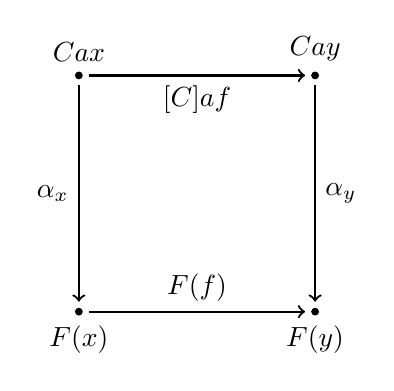
\begin{tikzpicture}[ele/.style={fill=black,circle,minimum
        width=.8pt,inner sep=1pt},every fit/.style={ellipse,draw,inner
        sep=-2pt}]

    % the texts
    \node[ele,label=above:$\catmsetfig{C}{a}{x}$] (cx) at (0,3) {};
    \node[ele,label=below:$F(x)$] (fx) at (0,0) {};
    \node[ele,label=above:$\catmsetfig{C}{a}{y}$] (cy) at (3,3) {};
    \node[ele,label=below:$F(y)$] (fy) at (3,0) {};

    \draw[->,thick,shorten <=2pt,shorten >=2pt] (cx) to
    node[below]{$\catmset[C]{a}{f}$} (cy);
    \draw[->,thick,shorten <=2pt,shorten >=2pt] (fx) to
    node[above]{$F(f)$} (fy);
    \draw[->,thick,shorten <=2pt,shorten >=2pt] (cx) to
    node[left]{$\alpha_x$} (fx);
    \draw[->,thick,shorten <=2pt,shorten >=2pt] (cy) to
    node[right]{$\alpha_y$} (fy);
  \end{tikzpicture}
  \caption{Commutative diagram for components of natural
    transformation $\alpha_x$ and $\alpha_y$}
  \label{fig:yoneda_proof_commutative_diagram}
\end{figure}

Functor
$\catcovhom{C}{a}$ maps $x$ into $\catmset[C]{a}{x}$ and $y$ into 
$\catmset[C]{a}{x}$. Functor $F$ maps the 2 objects into $F(x)$ and
$F(y)$ respectively. There is a \mynameref{def:nt} $\alpha$ between
the functors. I.e.  $\alpha \in
\catmset[\funcat{C}{Set}]{\catcovhom{C}{a}}{F}$. We are interested in
2 components of the natural transformations:
\[
\alpha_x : \catmset[C]{a}{x} \to F(x)
\]
and
\[
\alpha_y : \catmset[C]{a}{y} \to F(y).
\]
The components of natural transformation should satisfy the naturality
conditions \eqref{eq:nt_definition} i.e. the commutative diagram
\cref{fig:yoneda_proof_commutative_diagram} should commute.

We can replace object $x$ with $a$ in $\catmset[C]{a}{x}$. The result
set $\catmset[C]{a}{a}$ should contain \mynameref{def:id} $\idm{a}$.
Lets look how the morphism is mapped by the commutative diagram from
\cref{fig:yoneda_proof_commutative_diagram}.

\begin{figure}
  \centering
  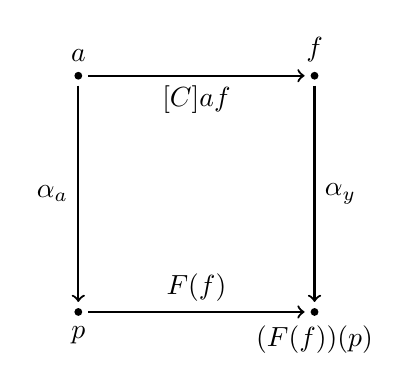
\begin{tikzpicture}[ele/.style={fill=black,circle,minimum
        width=.8pt,inner sep=1pt},every fit/.style={ellipse,draw,inner
        sep=-2pt}]

    % the texts
    \node[ele,label=above:$\idm{a}$] (cx) at (0,3) {};
    \node[ele,label=below:$p$] (fx) at (0,0) {};
    \node[ele,label=above:$f$] (cy) at (3,3) {};
    \node[ele,label=below:$(F(f))(p)$] (fy) at (3,0) {};

    \draw[->,thick,shorten <=2pt,shorten >=2pt] (cx) to
    node[below]{$\catmset[C]{a}{f}$} (cy);
    \draw[->,thick,shorten <=2pt,shorten >=2pt] (fx) to
    node[above]{$F(f)$} (fy);
    \draw[->,thick,shorten <=2pt,shorten >=2pt] (cx) to
    node[left]{$\alpha_a$} (fx);
    \draw[->,thick,shorten <=2pt,shorten >=2pt] (cy) to
    node[right]{$\alpha_y$} (fy);
  \end{tikzpicture}
  \caption{Mapping for $\idm{a}$. The identity morphism is mapped into
    $p \in F(a)$ i.e. $p = \alpha_a(\idm{a})$}
  \label{fig:yoneda_proof_idm}
\end{figure}

As we can see in \cref{fig:yoneda_proof_idm}, morphism $\alpha_a$
pick up an element $p$ of the set $F(a)$. There is an arbitrary
element that is determined by $\alpha_a$. All others elements in
\cref{fig:yoneda_proof_idm} is completely determined by the choice of
$p$. From \cref{def:cov_hom_functor} we have
\[
\catmset[C]{a}{f} = \{f \circ g | g \in \catmset[C]{a}{x}\}
\]
i.e. if $g = \idm{a}$ then 
\[
\catmset[C]{a}{f}\left(\idm{a}\right) = f
\circ \idm{a} = f.
\]
From other side we have mapping $F(f): p \to q$ where 
$q = (F(f))(p)$. I.e. if we pick an arbitrary object $y \in \catob{C}$
when we can pick a morphism $f: a \to y$. This leads to the definition
for an arbitrary component $\alpha_y$ of \mynameref{def:nt} $\alpha$
as soon as only one component $\alpha_a$ is defined:
\[
\alpha_y(f) = (F(f))(p).
\]
Therefore from only one element $p \in F(a)$ we can got the
\mynameref{def:nt} $\alpha \in
\catmset[\funcat{C}{Set}]{\catcovhom{C}{a}}{F}$. We also can go in
other direction i.e. $\alpha_a(\idm{a})$ will gives as an element $p$
from the set $F(a)$.
\end{proof}
\end{lemma}

\section{Examples}

\subsection{Quantum mechanics}

\subsubsection{Flori interpretation of quantum mechanics}
TBD
